\documentclass{article}
\usepackage[utf8]{vietnam}
\usepackage{graphicx}
\usepackage{amsmath}
\usepackage{amssymb}
\usepackage{hyperref}
\usepackage{caption}
\usepackage{subcaption}

\title{A gentle introduction to Filtering in the Frequency Domain\\ \Large Report Lab Week 5-6 Part1}
\author{Ngọc Thuận - IPSAL LAB}
\date{December 2022}

\begin{document}
\maketitle
\begin{abstract}
    Trong những bài trước, chúng ta đã cùng nhau nhiên cứu những các phép biến đổi trên miền không gian (Spatial Domian), rất hiển hiện, rõ ràng. Trong bài này, ta sẽ nghiên cứu về các phép biến đổi trên miền tần số (Frequency Domain), một miền `vô hình' hơn, và cũng rất thú vị! Trong đó, ta sẽ tìm hiểu về cơ sở toán học của phép biến đổi Fourier (Fourier Transform), đưa tín hiệu/ảnh sang miền tần số như thế nào. Và biết thêm một số phép biến đổi mới, trên miền tần số, dựa trên những nền tảng trên!
\end{abstract}
\tableofcontents


\newpage

\section{Introduction}
    \subsection{Giới thiệu}
    \textit{Phép biến đổi Fourier} là không còn quá mới mẻ, nhưng lại vô cùng quan trọng trong khoa học hiện đại, có thể kể đến như: vật lý, số học, xử lí tin hiệu, xác suất, thống kê, mật mã, âm học, hải dương học, quang học, hình học, \ldots. Được đặt tên theo nhà toán học có đóng góp lớn cho nó: \href{https://en.wikipedia.org/wiki/Joseph_Fourier}{Joseph Fourier}
     (21 March 1768 - 16 May 1830). 
     \begin{figure}[ht!]
        \centering
        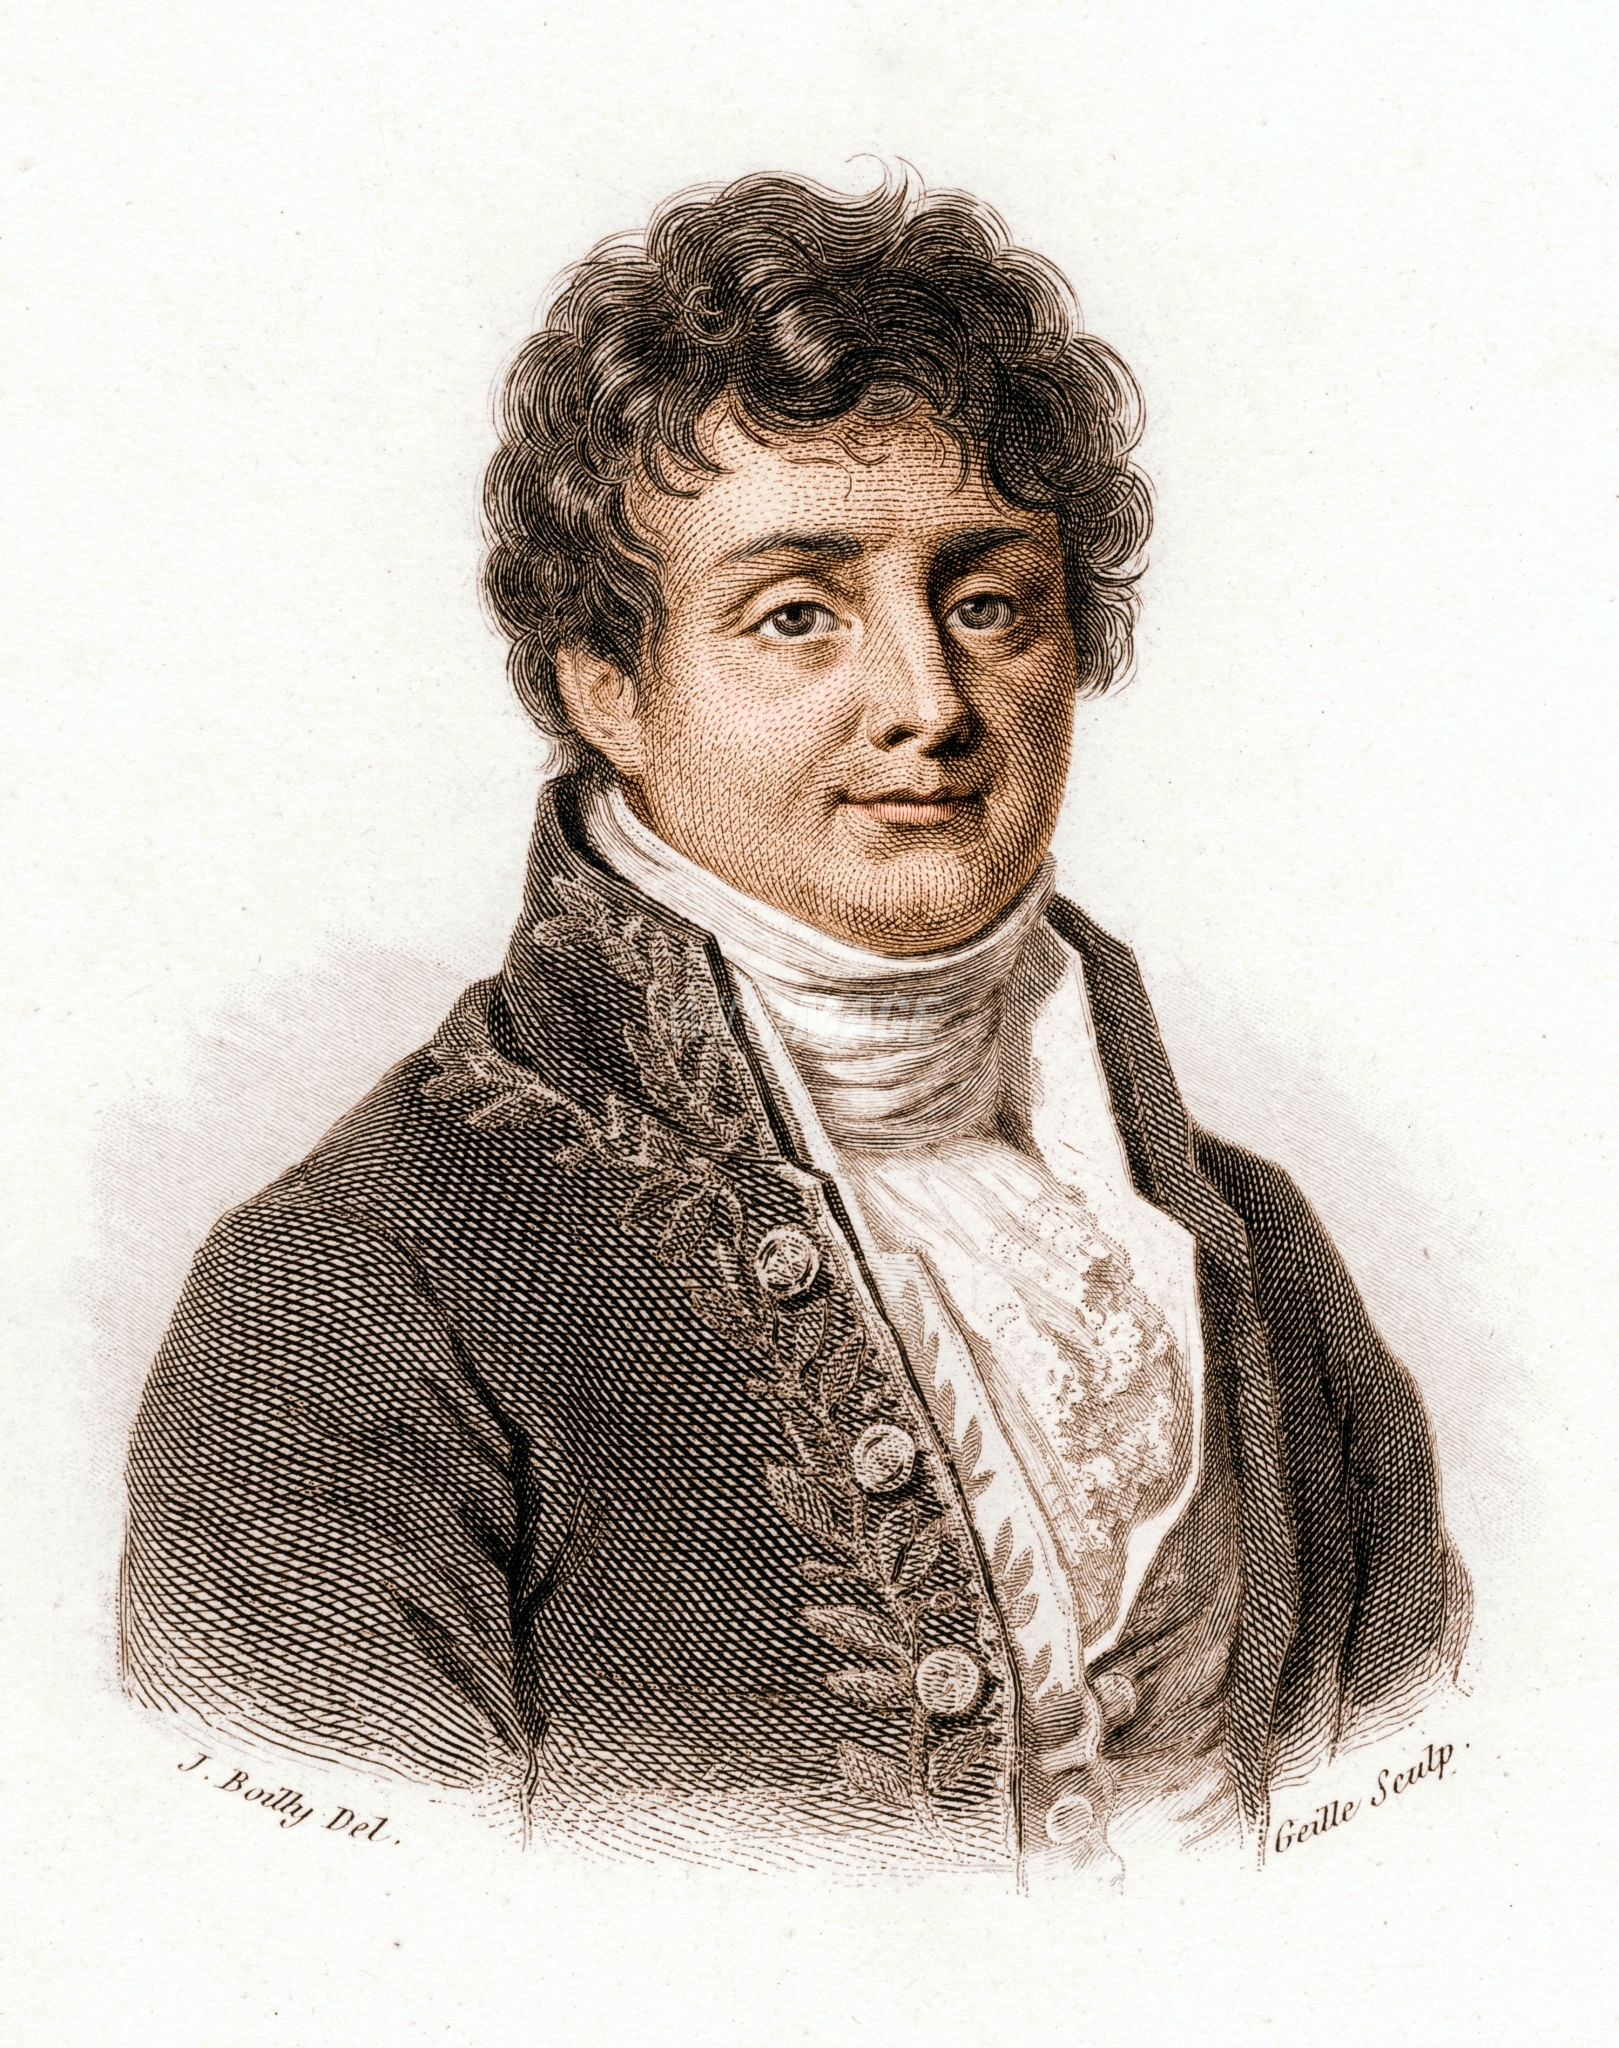
\includegraphics[width = 0.4\linewidth]{Fourier.jpg}
        \caption{\textbf{Jean-Baptiste Joseph Fourier} (21 March 1768 - 16 May 1830)}
        \label{fig1}
     \end{figure}
     Với ý tưởng đột phá là đưa hàm số trên miền thời gian về miền tần số, và ngược lại!\\
    Ban đầu không mấy ai để ý đến công trình trên, nhưng thời gian đã đã chứng minh tầm quan trọng ấy. Từ một dạng cơ bản sau đó là nhiều dạng khác của \textit{Biến đổi Fourier} ứng dụng trong vô vàn lĩnh lực trong cuộc sống!\\
    Trong bài này tôi sẽ giới thiệu sơ lược về \textit{Phép biến đổi Fourier} liên tục, rời rạc và một số thuật toán hiện đại với \textit{Phép biến đổi Fourier}! \\Nhưng trước khi làm việc với những thứ trên, hãy có cái nhìn sơ qua về nguồn gốc của \textit{Phép biến đổi Fourier}!
    \subsection{Fourier Series}
    \textit{Chuỗi Fourier}, một thành tựu cũng vô cùng to lớn của \textit{Fourier}! Với ý tưởng đơn giản ban đầu đó là `xấp xỉ' một hàm số tuần hoàn thành tổng vô hạn các hàm \textit{sine} và \textit{cosine}.
    \begin{figure}[ht!]
        \centering
        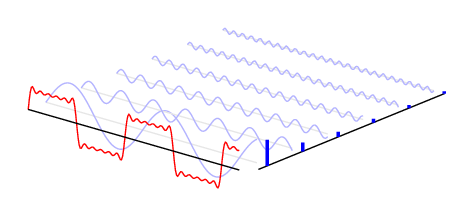
\includegraphics[width = 0.7\linewidth]{fourier-series.png}
        \caption{Ý tưởng đơn giản của chuỗi Fourier}
        \label{fig2}
     \end{figure}
        \subsubsection{Định nghĩa}
        \fbox{
        \begin{minipage}{\linewidth}
        Giả sử $f$ là một hàm số tuần hoàn xác định trên $\mathbb{R}$ với chu kì $T$, liên tục từng khúc trên mỗi đoạn bị chặn. Chuỗi lượng giác
        \begin{equation}
        \frac{a_0}{2}+\sum_{n=1}^{\infty} a_n \cos n\omega x + b_n \sin n\omega x  
        \label{eq1}
        \end{equation}

        trong đó các hệ số được cho bởi các công thức: \\ \\
        $a_0 = \frac{2}{T} \int_{-T/2}^{T/2} f(t) dt $\\ \\
        $a_n = \frac{2}{T} \int_{-T/2}^{T/2} f(t) \cos n\omega t dt$ \\ \\
        $b_n = \frac{2}{T} \int_{-T/2}^{T/2} f(t) \sin n\omega t dt$ \\ \\
        gọi là \textit{chuỗi Fourier} của hàm số $f$. $a_n, b_n$
     được gọi là các \textit{hệ số Fourier}.\\ \\ Với $\omega = \frac{2\pi}{T}.$\\    \end{minipage}
        }\\ \\
        Đó là phát biểu gốc, và vô cùng chặt chẽ về mặt toán học. Song, cái nhìn này chưa cho ta cái mà chúng ta cần.\\
        Thật vậy, ta sẽ phát biểu (\ref{eq1}) dưới dạng khác đi một chút! Đó là dạng phức của \textit{chuỗi Fourier}!!! 
        \subsubsection{Dạng phức của chuỗi Fourier - Complex form of Fourier Series}
        Từ (\ref{eq1}) và các công thức \textit{Euler} cho \textit{sin} và \textit{cos}, ta có:
        $$ f(x) = \frac{a_0}{2} + \sum_{n=1}^{\infty} \left[a_n \left(\frac{e^{jn\omega x}+e^{-jn\omega x }}{2} \right) + b_n \left(\frac{e^{jn\omega x}-e^{-jn\omega x }}{2j} \right) \right] $$

        $$ f(x) = \frac{a_0}{2} + \sum_{n=1}^{\infty} \left(\frac{a_n - jb_n}{2}\right)e^{jn\omega x}+\sum_{n=1}^{\infty} \left(\frac{a_n + jb_n}{2}\right)e^{-jn \omega x}$$
        Đặt $c_n = \frac{1}{2} \left(a_n - jb_n \right), n = 1, 2, \ldots$, tương tự $\bar{c}_n = \frac{1}{2} \left(a_n + jb_n \right), n = 1, 2, \ldots$\\ \\
        Sau đó, đặt $k = -n$, ta có:
        $$f(x) = \frac{a_0}{2} + \sum_{n=1}^{\infty} {c_n}e^{-jn\omega x}+\sum_{k=-1}^{-\infty} {\bar{c}_k}e^{jk \omega x}$$
        Mở rộng hàm số, cho $c_n = \bar{c}_n , n = -1, -2, \ldots$ và $c_0 = a_0/2$. Ta có thể tóm gọn lại được chuỗi Fourier như sau:
        \begin{equation}
            \fbox{$f(x) = \sum_{-\infty}^{\infty} c_n e^{jn\omega x}, n \in \mathbb{Z}$}
        \label{eq2}
        \end{equation}
        và 
        \begin{equation}
            \fbox{$c_n = \frac{1}{T} \int_{-\frac{T}{2}}^{\frac{T}{2}} f(x) e^{-jn\omega x} dx$}
            \label{eq3}
        \end{equation}

        (\ref{eq2}) và (\ref{eq3}) chính là dạng phức của \textit{Chuỗi Fourier}. Khi ở dạng phức ta có nhận xét sau:
        \begin{enumerate}
            \item $c_n$ là hàm biến phức phụ thuộc vào $\omega$.
            \item $c_n$ là \textit{số phức} tạo bởi tổng hợp hai thành phần \textit{sin, cos} cùng tần số. 
            \item Module của $c_n$ chính là biên độ dao động tại tần số $\omega$ cho trước.
        \end{enumerate}
        \subsubsection{Từ Fourier Series đến Fourier Transform.}
        \label{n1}
        \underline{Nhận xét}: Ta có thể coi một hàm không tuần hoàn là một hàm tuần hoàn với chu kì rất rất lớn!\\
        Đặt $\mu = n/T$ và $F(\mu) = T c_n$. \\
        \textbf{Với $T$ rất lớn ($f$ không tuần hoàn), ta coi $T = \infty$}. Khi đó (\ref{eq3}) trở thành:
        \begin{equation}
            F(\mu) = \int_{-\infty}^{\infty} f(x) e^{-j2\pi \mu x} dx
            \label{eq4}
        \end{equation}
        Bên cạnh đó, (\ref{eq2}) tương đương:
        \begin{equation}
            f(x) = \sum_{-\infty}^{\infty} Tc_n e^{j2\pi \frac{n}{T} x} \frac{1}{T} = \int_{-\infty}^{\infty} F(\mu) e^{j2\pi \mu x} d\mu
            \label{eq5}
        \end{equation}
        Công thức (\ref{eq4}) cho ta \textit{Phép biến đổi Fourier} cho một hàm số bất kì (không nhất thiết phải tuần hoàn).\\
        Và, công thức (\ref{eq5}) cho ta \textit{Phép biến đổi Fourier ngược}.
        \subsection{Fourier Transform}
        \subsubsection{Định nghĩa}
        Tôi đã chứng minh một cách sơ qua \textit{Phép biến đổi Fourier} từ \textit{Chuỗi Fourier} (\textit{xem lại phần \ref{n1}}). Bây giờ ta sẽ định nghĩa nó một cách rõ ràng:\\
        \fbox{
        \begin{minipage}{\linewidth}
        Nếu tín hiệu $f(t)$ không nhất thiết tuần hoàn, thỏa mãn:
        \begin{enumerate}
            \item $\int_{-\infty}^{\infty} |f(t)|< \infty$, tức là $\int_{-\infty}^{\infty} |f(t)|$ hội tụ.
            \item $f(t)$ trong khoảng hữu hạn bất kì liên tục từng khúc.
            \item Tại điểm không liên tục $t_0$ thỏa mãn $f(t_0) = \frac{1}{2}\left[x(t_0-0)+x(t_0+0)\right]$.
            \item $f(t)$ trong khoảng hữu hạn bất kì chỉ có hữu hạn các điểm cực trị.

        \end{enumerate}
        thì $f(t)$ biểu diễn được dưới dạng \textit{tích phân Fourier} như sau:
        \begin{equation}
            F(\mu) = \int_{-\infty}^{\infty} f(t) e^{-j2\pi \mu t} dt
            \label{eq6}
        \end{equation}
        và,
        \begin{equation}
            f(t) =  \int_{-\infty}^{\infty} F(\mu) e^{j2\pi \mu t} d\mu
            \label{eq7}
        \end{equation}
        \end{minipage}
        }
        \subsubsection{Tính chất}
        \label{n2}
        \textit{Phép biến đổi Fourier} có nhiều tính chất, nhưng cơ bản nhất:
        \begin{enumerate}
            \item \textit{Tính tuyến tính}: $F(ax(t)+by(t)) = aX(\mu)+bY(\mu)$. Đây là lí do \textit{Phép biến đổi Fourier} cũng được gọi là \textit{Toán tử Fourier}!
            \item \textit{Fourier} của tích chập bằng tích các \textit{Fourier}:
            $F(x(t)*y(t)) = X(\mu) Y(\mu)$
        \end{enumerate}
        vân vân, \ldots.\\Tính chất số 2, là lí do ta có bài này, và nhiều trò khác trong xử lí tín hiệu, chúng ta sẽ đề cập đến trong phần (ref).\\
        Tìm hiểu thêm tại \href{https://en.wikipedia.org/wiki/Fourier_transform}{Fourier Transform}.
        \subsubsection{Fourier Spectrum and Phase Angle}
        Ta có thể tách \textit{Phép biến đổi Fourier} thành một hàm biến phức từ công thức \textit{Euler}, như sau:
        $$ F(\mu) = R(\mu) + jI((\mu)$$
        $|F(\mu)| = \left(R^{2}(\mu)+I^{2}(\mu)\right)^{1/2}$ : Fourier Spectrum\\ \\
        $\phi(\mu) = \arctan \frac{I(\mu)}{R(\mu)}$: Phase Angle.
        \\ \\
         $|F(\mu)|^2 = R^{2}(\mu)+I^{2}(\mu)$: Power Spectrum. Hình \ref{fig3}.
        \begin{figure}[ht!]
        \centering
        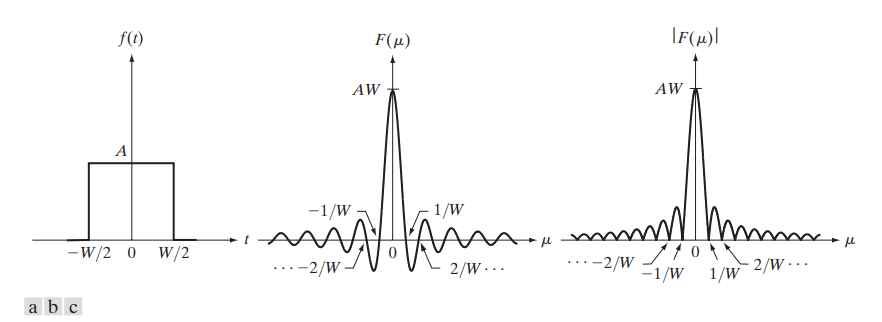
\includegraphics[width = \linewidth]{fo1.png}
        \caption{(a) A simple function; (b) its Fourier transform; and (c) the spectrum.}
        \label{fig3}
        \end{figure}
        \subsubsection*{Nhận xét}
        Như tôi đã nói lúc giới thiệu \textit{Phép biến đổi Fourier} cho phép ta chuyển đổi qua lại giữa miền tần số và miền thời gian của một tín hiệu. Hiển nhiên qua đây ta có cái nhìn đa chiều về một tín hiệu theo cả nghĩa đen lẫn nghĩa bóng, đồng thời mở rộng khái niệm tần số ra không chỉ trong vật lí, mà trong mọi tín hiệu trong cuộc sống! \\Hình \ref{fig4}, minh họa cho góc nhìn của chúng ta trên cùng một tín hiệu, trong những miền không gian khác nhau!
        \begin{figure}[ht!]
        \centering
        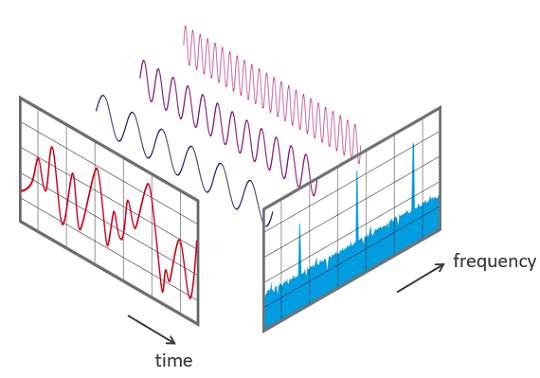
\includegraphics[width = 0.7\linewidth]{fo2.png}
        \caption{Phép biến đổi Fourier cho ta cái nhìn đa chiều về một tín hiệu (cả miền thời gian và tần số).}
        \label{fig4}
        \end{figure}
        \\
        Trong xử lí ảnh đôi khi với việc sử dụng các bộ lọc không gian lại trở nên khó khăn, đặc biệt trong những trường hợp ảnh lớn! Khi đó bộ lọc không gian tỏ ra chậm chạp, thiếu hiệu quả. Thì với tích châp của \textit{Phép biến đổi Fourier} (\textit{phần \ref{n2}}), và những đột phá trong thuật toán \textit{Biến đổi Fourier nhanh (FFT)} thì đây là một điểm cộng!\\
        Ngoài ra, \textit{Biến đổi Fourier} cũng tỏ ra chẳng hề kém cỏi trong các công việc khử nhiễu và khôi phục ảnh,\ldots (\textit{tí nữa ta sẽ bàn luận sâu hơn về vấn đề này!})
        
        \subsection{Biến đổi Fourier rời rạc - Discrete Fourier Transform}
        \subsubsection*{Biến đổi Fourier rời rạc thuận - DFT}
        Ở mục \ref{n1}, ta đã nhìn thấy rằng, xuất phát điểm của \textit{Phép biến đổi Fourier} xuất phát từ \textit{Chuỗi Fourier}. Mà tần số của \textit{Chuỗi Fourier} lại là các điểm không liên tục! Cho nên phần này ta như đi ngược lại, lật lại kiến thức!\\
        Giả sử cho một tín hiệu rời rạc $f = [f_0, f_1,\ldots, f_{M-1}]$. Độ dài M.\\
        Mở rộng $f$ thỏa mãn:
        \begin{equation}
            f = 
            \begin{cases}
            f_i\quad, if \phantom{r}i \in [0, M-1]\\
            0\quad, otherwise
            \end{cases}
        \end{equation}
        \\Trong phần trước tôi đã đặt $\mu = n/T$, $T$ được coi là rất lớn, nhưng trong trường hợp này, $T$ lớn nhất chỉ có thể là $M$.\\
        Vậy, đặt $T = M$. Thay vào công thức ta có:
        \begin{equation}
        F(n) = \sum_{x=0}^{M-1}f(x)e^{-j2\pi \frac{n}{M}x}, n = 1, 2, \ldots, M
        \label{eq9}
        \end{equation}
        \\ Thông thường thì chúng ta sử dụng:
                \begin{equation}
        F(n) = \sum_{x=0}^{M-1}f(x)e^{-j2\pi \frac{n}{M}x}, n = 0, 1, \ldots, M-1
        \label{eq10}
        \end{equation}
        \\ thay vì (\ref{eq9}).\\
        \subsubsection*{Biến đổi Fourier rời rạc ngược - IDFT}
        Một cách tương tự, 
        \begin{equation}
            f(x) = \frac{1}{M}\sum_{n=0}^{M-1} F(n)e^{j2\pi nx/M}, x = 0, 1, 2, \ldots, M-1
        \end{equation}
        Như đã thấy, tất cả các công thức trên, là áp dụng cho trường hợp một chiều (chủ yếu là miền thời gian), và việc đó là khó khăn nếu muốn áp dụng trong các miền khác nhiều chiều hơn, ví dụ ngay là miền không gian. Vậy nên, việc mở rộng \textit{Phép biến đổi Fourier} là cần thiết! Sau đây ta sẽ đi tìm hiểu về \textit{Phép biến đổi Fourier hai chiều}!
        \subsection{Biến đổi Fourier rời rạc hai nhiều - Discrete Fourier Transform in 2D Case}
        \subsubsection{Phép biến đổi Fourier liên tục hai chiều - 2D Continous Fourier Transform}
        Ta định nghĩa \textit{Phép biến đổi Fourier} liên tục hai chiều tổng quát như sau:\\
        \fbox{
        \begin{minipage}{ \linewidth}
        Thuận:
        \begin{equation}
            F(u,v) = \int_{-\infty}^{\infty} \int_{-\infty}^{\infty} f(x,y) e^{-j2\pi (ux+vy)} dx dy
            \label{eq12}
        \end{equation}
        Ngược:
        \begin{equation}
            f(x,y) = \int_{-\infty}^{\infty} \int_{-\infty}^{\infty} F(u,v) e^{j2\pi (ux+vy)} du dv
            \label{eq13}
        \end{equation}
        \end{minipage}
        }
        \subsubsection{Phép biến đổi Fourier rời rạc hai chiều - 2D Discrete Fourier Transform}
        \fbox{
        \begin{minipage}{ \linewidth}
        Thuận:
        \begin{equation}
            F(u,v) = \sum_{x=0}^{M-1} \sum_{y=0}^{N-1} f(x,y) e^{-j2\pi (ux/M+vy/N)},
            \label{eq14}
        \end{equation}
         $$ u = 0, 1, \ldots, M-1; \phantom{abcd} v = 0, 1, \ldots, N-1$$
         Ngược:
        \begin{equation}
            f(x,y) = \frac{1}{MN} \sum_{u=0}^{M-1} \sum_{v=0}^{N-1} F(u,v) e^{j2\pi (ux/M+vy/N)},
            \label{eq15}
        \end{equation}
        $$x = 0, 1, \ldots, M-1;\phantom{abcd} y = 0, 1, \ldots N-1$$
        \end{minipage}
        }
        \subsubsection*{Lưu ý}
        Giả sử phổ ban đầu được chia thành 4 góc phần tư (Hình \ref{fig5}, trái) thì các góc sẽ là những thành phần có tần số thấp nhất. Trong đó $F(0,0)$ đôi khi được gọi là \textit{thành phần DC} (\textit{DC component}) của ảnh, ẩn dụ cho việc `không' tần số của nó.
        \begin{figure}[ht!]
        \centering
        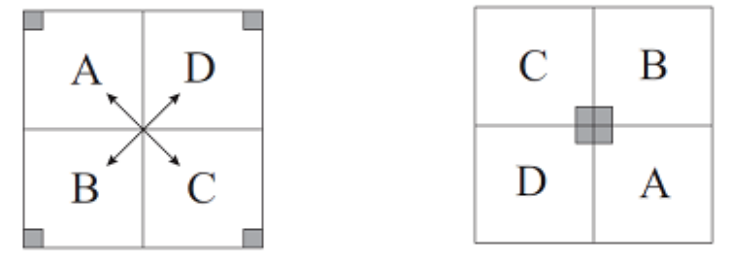
\includegraphics[width = 0.5\linewidth]{fo3.png}
        \caption{Original spectrum low frequencies in corners (left), Shifted spectrum with the origin at (M/2, N/2) (right)}
        \label{fig5}
        \end{figure}
        \\ Thông thường, ta sẽ hoán đổi các mảnh để được các điểm có tần số thấp ở giữa, dựa trên tính đối xứng của phổ!.\\
        Ta muốn các điểm có tần số thấp vào tâm của miền, do đó, yêu cầu bài toán tương đương: \textit{Tìm hàm số $g$ sao cho $G(u,v) = F(u-M/2,v-N/2)$}.\\
        Thật vây, ta có:
        $$F(u-M/2, v-N/2) = \sum_{x=0}^{M-1} \sum_{y=0}^{N-1} f(x,y) e^{-j2\pi (ux/M+vy/N-(x+y)/2)},$$
        Tương đương,
        $$F(u-M/2, v-N/2) = \sum_{x=0}^{M-1} \sum_{y=0}^{N-1} f(x,y) e^{j\pi(x+y)} e^{-j2\pi (ux/M+vy/N)} 
        $$
        $$\phantom{F(u-M/2, v-N/2)} = \sum_{x=0}^{M-1} \sum_{y=0}^{N-1} f(x,y) (-1)^{x+y} e^{-j2\pi (ux/M+vy/N)}$$
        Suy ra, \fbox{$g(x,y) = f(x,y) (-1)^{x+y}$}. Hàm số này sẽ cho ta kết quả như Hình \ref{fig5} (phải).\\ \\
        \begin{figure}[ht!]
        \centering
        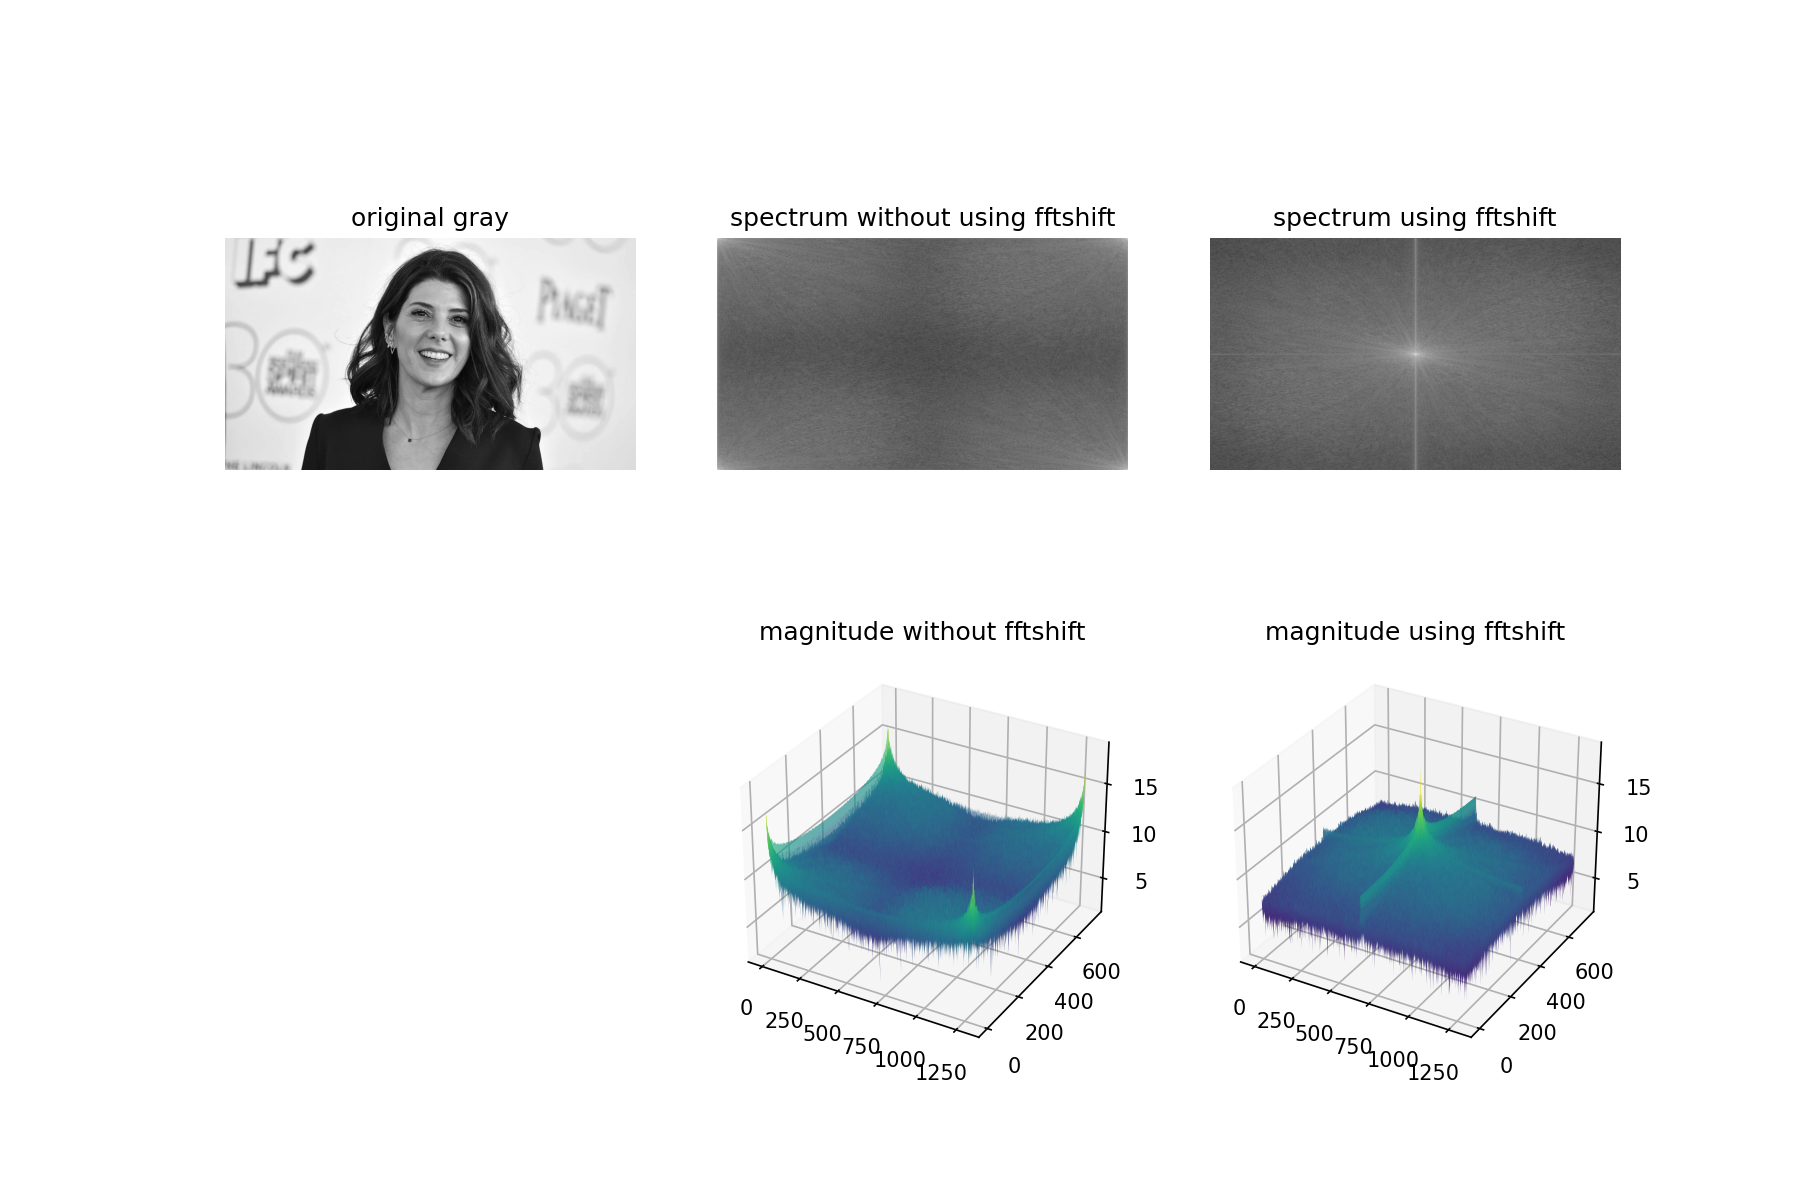
\includegraphics[width = 0.9\linewidth]{fo5.png}
        \caption{Fourier Transform của ảnh}
        \label{fig7}
        \end{figure}
        Bên cạnh những điều trên, ta còn có những khái niệm vô cùng thú vị về tính chẵn lẻ, đối xứng, liên hợp đối xứng,\ldots (Hình \ref{fig6}). Tôi định viết, nhưng cũng thấy trong phạm vi bài này cũng không dùng đến và chúng ta cũng đã khá lan man trong bài này rồi. Nên xin nhường lại bạn đọc tự tìm hiểu, nếu có thời gian, tôi sẽ bổ sung chi tiết hơn!
        \begin{figure}
        \centering
        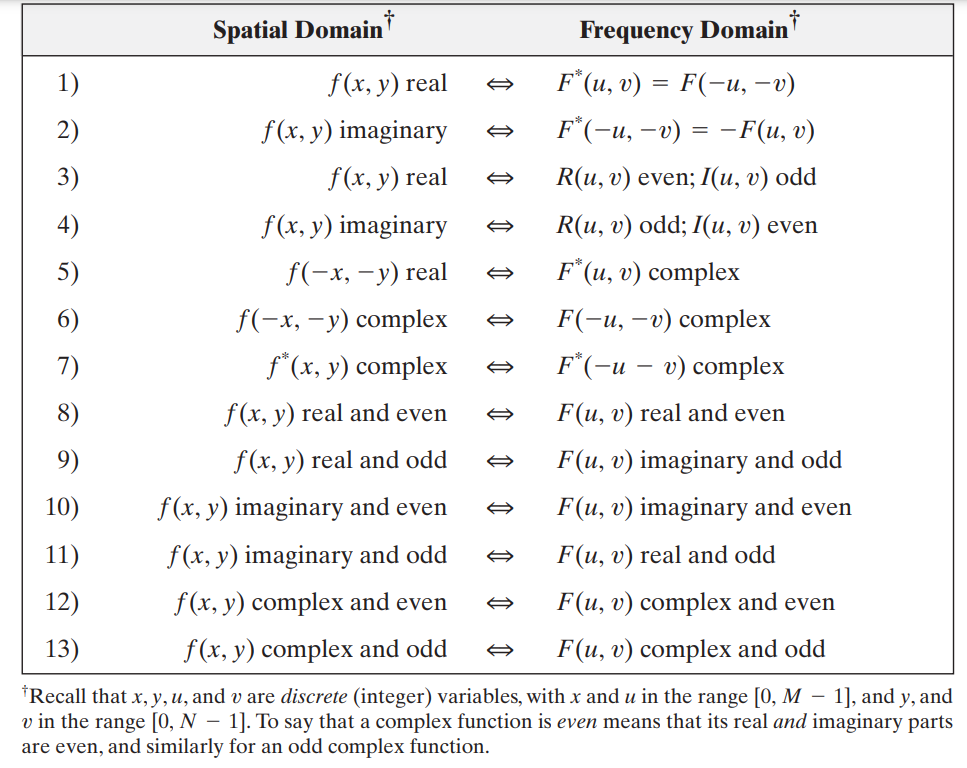
\includegraphics[width = \linewidth]{fo4.png}
        \caption{Some symmetry properties of the 2D DFT and its inverse. $R(u,v)$ and $I(u,v)$ are the real and imaginary parts of $F(u,v)$ respectively. The tearm \textit{complex} indicates that a funtion has nonzero real and imaginary parts.}
        \label{fig6}
        \end{figure}
        
        \subsection{Thuận toán biến đổi Fourier nhanh - Fast Fourier Transform (FFT)}
        \section{Filtering in the Frequency Domain}
        \subsection{The basics of filtering in the frequency domain}
        \begin{figure}[ht!]
            \centering
            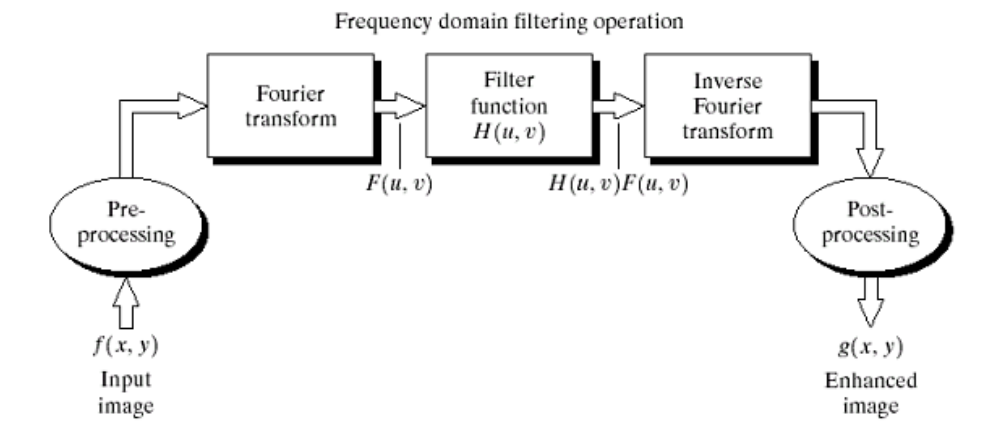
\includegraphics[width = 0.7\linewidth]{fo6.png}
            \caption{Frequency domain filtering operation}
            \label{fig8}
        \end{figure}
        Hìnnh \ref{fig8} cho ta thấy các thao tác cơ bản của lọc trong miền tần số.\\
        Tuy nhiên, ta có thể đơn giản hơn nữa sơ đồ trên chỉ với 3 bước:
        \begin{enumerate}
            \item Tính $F(u,v)$, `ảnh' của ảnh trong miền tần số (\textit{DFT of the image})
            \item Nhân $F(u,v)$ bởi bộ lọc $H(u,v)$
            \item Tính Fourier ngược của kết quả (\textit{inverse DFT - IDFT})
        \end{enumerate}
        \underline{Chú ý}: Nên đệm ảnh (\textit{padding}) trước khi chuyển ảnh sang miền tần số. Có thể do một số lí do như sau:
        \begin{enumerate}
            \item Nếu để ý, khi ta đưa \textit{Phép biến đổi Fourier} từ liên tục sang rời rạc, $T=M$, như đã biết $T$ trong miền liên tục, là một số `rất lớn' hiển nhiên với $M$ lớn sẽ cho kết quả tốt hơn đã đành. Nhưng bên cạnh đó, việc \textit{zero-padding} hầu như không ảnh hưởng đến tổng, nhưng lại tăng độ sấp xỉ giữa tín hiệu rời rạc và liên tục (\textit{nội suy}) (\textit{giống tăng thời gian trích mẫu}). Và điều này làm cho kết quả của ta càng trở nên chính xác về mặt lí thuyết.
            \item Thứ hai, trong miền tần số, phép tích chập không còn là khó khăn với ta, vì nó chỉ đơn giản là phép nhân, thay vì phải trượt lên trượt xuống như miền không gian. Cho nên, khi \textit{padding}, thường ta sẽ \textit{padding} với số lượng tương đối lớn mà không sợ, ảnh hưởng đến thời gian thực hiện!
            \item Cuối cùng, khi ta tăng kích thước bằng \textit{zero-padding}, bên cạnh ảnh gốc, thì \textit{hàm truyền} của ta cũng sẽ thay đổi kích thước, hiển nhiên với kích thước lớn hơn, toán tử sẽ mang được nhiều thông tin, phép biến đổi hơn vào bức ảnh!
        \end{enumerate}
        \begin{figure}[ht!]
            \centering
            \begin{subfigure}[b]{0.4\linewidth}
                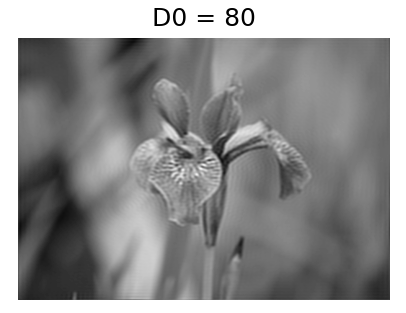
\includegraphics[width=\linewidth]{fo8.png}
                \caption{Không zero-padding}
            \end{subfigure}
            \begin{subfigure}[b]{0.4\linewidth}
                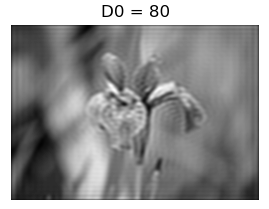
\includegraphics[width=\linewidth]{fo7.png}
                \caption{Có zero-padding}
            \end{subfigure}
            \caption{Minh họa cho kết quả khi padding và không padding}
            \label{fig9}
        \end{figure}
            Hình \ref{fig9}, cho ta cùng một hình ảnh khi được thực hiện cùng một phép biến đổi, hình (a) ta làm trực tiếp lên ảnh, hình (b) ta đã \textit{zero-padding} thành ảnh có kích thước gấp đôi ảnh ban đầu. Không khó để nhận ra sự khác biệt này!

            
        \subsubsection*{Trường hợp kích thước ảnh khác kích thước bộ lọc không gian}
        Giả sử ta có ảnh $f(x,y)$ có kích thước $A\times B$ và bộ lọc.\\
        Khi đó ta sẽ \textit{padding} vào ảnh và \textit{kernel} sao cho chúng có cùng kích thước là $P \times Q$ thỏa mãn $P \geq A+C-1$ and $Q \geq B+D-1$.\\
        Sau đó làm tương tự các bước trên.\\
        \underline{Chú ý}: Nên chọn P, Q sao cho P, Q là các lũy thừa bậc 2 (\textit{dựa trên kiến trúc máy tính}). 
        \subsection{Low-Pass Filtering}
        \textit{Low-Pass Filtering} - \textit{Lọc thông-thấp}, tức sẽ để các tần số thấp đi qua và bỏ đi những tần số cao. Cái tên cho ta ý tưởng của các phép biến đổi loại này! Ở bài trước, ta đã biết đến một bộ lọc thông-thấp, tuy nhiên lúc đó điều đó là không rõ ràng: Đó là bộ lọc \textit{Gauss}. Sau đây ta sẽ tìm hiểu một số bộ lọc thông-thấp thông dụng!
        \subsubsection{Ideal Low-Pass Filter}
        Hàm truyền của bộ thông thấp có thể biểu diễn dưới dạng toán học như sau:
        $$
        H(u,v) = \begin{cases}
            1, \phantom{a}if D(u,v) \leq D_0\\
            0,\phantom{a} if D(u,v) > D_0
        \end{cases}
        $$
        Với, $D(u,v)$ là khoảng cách từ tâm tới tọa độ tần số $(u,v)$. Nếu tâm là $(0,0)$. $D(u,v)$ có thể cho bới biểu thức:
        $$ D(u,v) = \left(u^2+v^2\right)^{1/2}$$
        \begin{figure}[ht!]
        \centering
        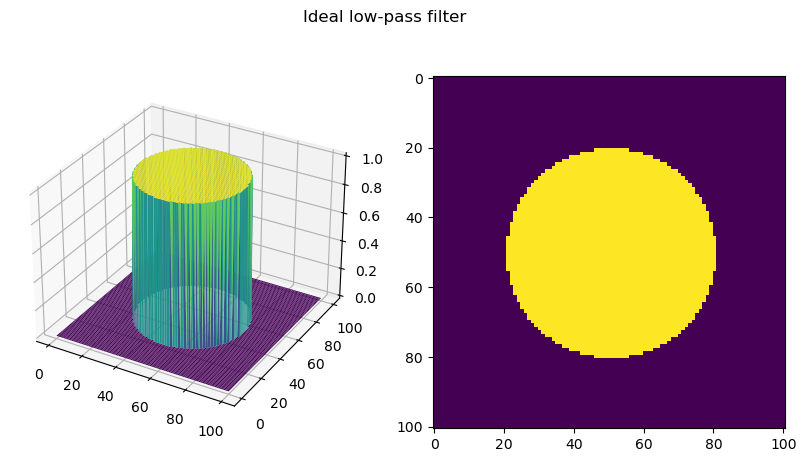
\includegraphics[width = \linewidth]{fo10.png}
        \caption{Ideal Low-Pass Filter}
        \label{fig11}
        \end{figure}
        Hình \ref{fig10} cho ta kết quả của \textit{Ideal Low-Pass Filtering}. (\textit{$D_0 = 80$ là ảnh được sử dụng để minh họa ở phần trên})
        \begin{figure}[ht!]
        \centering
        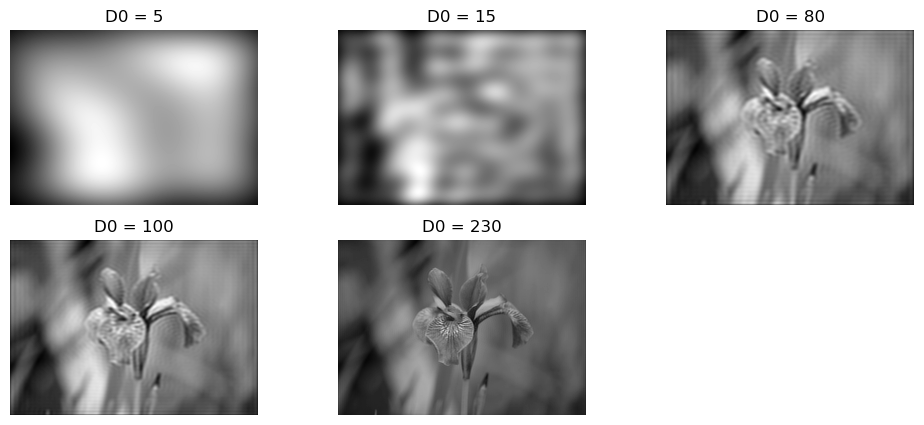
\includegraphics[width = \linewidth]{fo9.png}
        \caption{Kết quả của Ideal Low-Pass Filter, padding size*2}
        \label{fig10}
        \end{figure}
        
        \phantom{a}\\
        \textit{Ideal} - \textit{Lí tưởng}, vì nó thiếu đi nét mềm mại cần có, trong thực tế bộ lọc này ít được sử dụng!
        \subsubsection{Gaussian Low-Pass Filters}
        Hàm truyền có thể được cho bởi:
        $$H(u,v) = e^{-D^2(u,v)/2D_{0}^{2}}$$

        \begin{figure}[ht!]
        \centering
        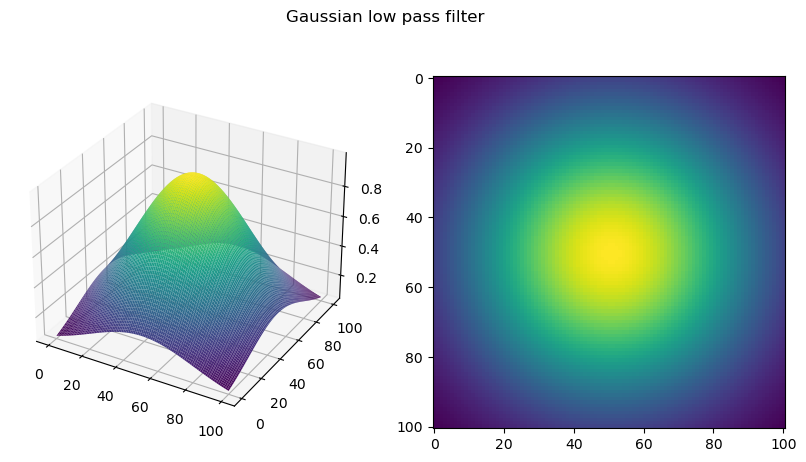
\includegraphics[width = \linewidth]{fo11.png}
        \caption{Gaussian Low-Pass Filtering}
        \label{fig12}
        \end{figure}
        Hình \ref{fig13} cho ta kết quả của \textit{Gaussian Low-Pass Filter}
        \begin{figure}[ht!]
        \centering
        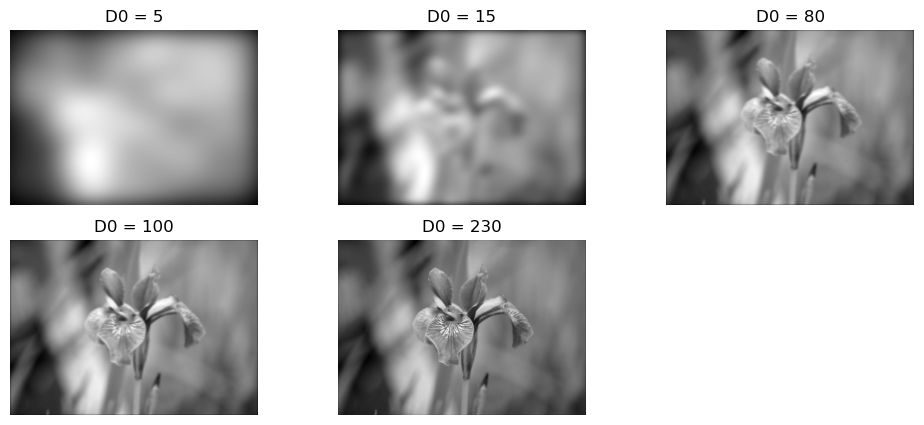
\includegraphics[width = \linewidth]{fo12.png}
        \caption{Kết quả của Gaussian Low-Pass Filter, padding size*2}
        \label{fig13}
        \end{figure}
        \phantom{a}\\
        Bộ lọc \textit{Gauss} thường được sử dụng để làm liền các văn bản bị vỡ, hoặc xóa đi các khuyết điểm (vết nhăn, \ldots) trước khi xuất bản.
        \begin{figure}[ht!]
            \centering
            \begin{subfigure}[b]{0.4\linewidth}
                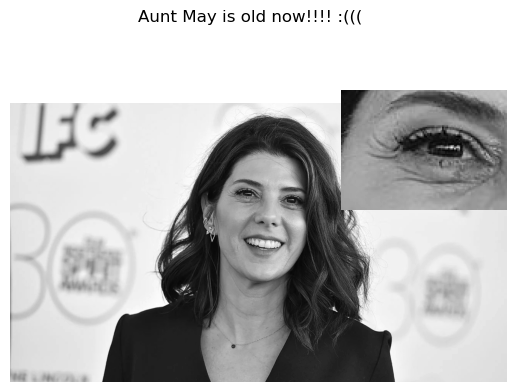
\includegraphics[width=\linewidth]{fo13a.png}
                \caption{Trước}
            \end{subfigure}
            \begin{subfigure}[b]{0.4\linewidth}
                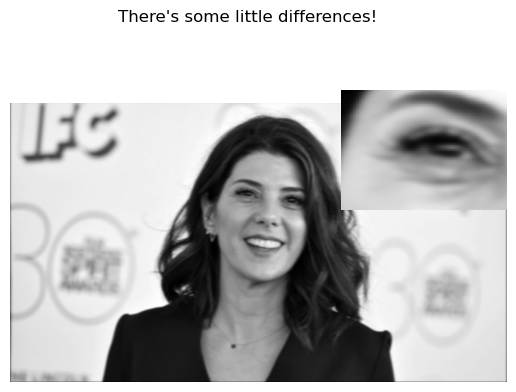
\includegraphics[width=\linewidth]{fo13b.png}
                \caption{Sau}
            \end{subfigure}
            \caption{Bộ lọc Gauss thường dùng để xóa những khuyết điểm.}
            \label{fig14}
        \end{figure}
        \begin{figure}[ht!]
        \centering
        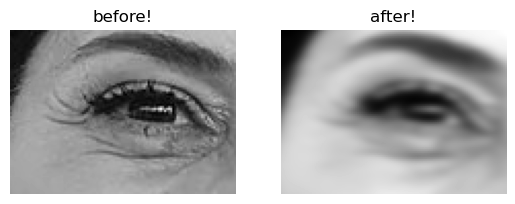
\includegraphics[width = 0.8\linewidth]{fo14.png}
        \caption{Trước và sau khi dùng Gauss.}
        \label{fig15}
        \end{figure}
        \subsubsection{Butterworth Low-Pass Filters}
        Hàm truyền có thể được cho bởi:
        $$ \frac{1}{1+\left[D(u,v)/D_{0} \right]^{2n}}$$
        Sự khác biệt giữa \textit{Butterworth Low-Pass Filters} và hai bộ lọc trước đó, bên cạnh công thức toán học và cái tên của tác giả thì đó còn là $n$ (\textit{the order n}). Đó cũng là điểm biến bộ lọc này hoàn toàn khác biệt: Nếu \textit{the order} càng lớn thì càng gần \textit{Ideal filter}, \textit{the order} càng nhỏ càng gần \textit{Gaussian filter}. Cho nên trong thực tế, người ta hay sử dụng \textit{Butterworth} cũng nhờ đặc tính đa năng này của nó!\\
        \begin{figure}[ht!]
        \centering
        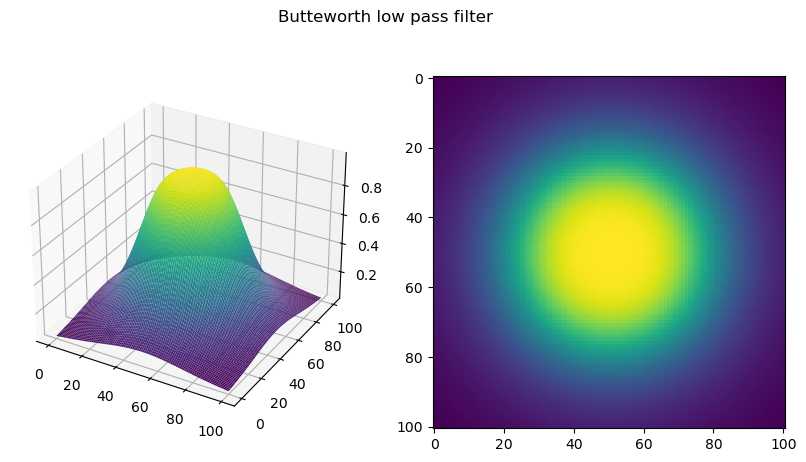
\includegraphics[width = \linewidth]{fo15.png}
        \caption{Butterworth Low-Pass Filter}
        \label{fig16}
        \end{figure}
        Hình \ref{fig17} cho ta kết quả của \textit{Butterworth Low-Pass Filtering} khi giữ cấp độ và thay đổi các khoảng cách.
        \begin{figure}[ht!]
        \centering
        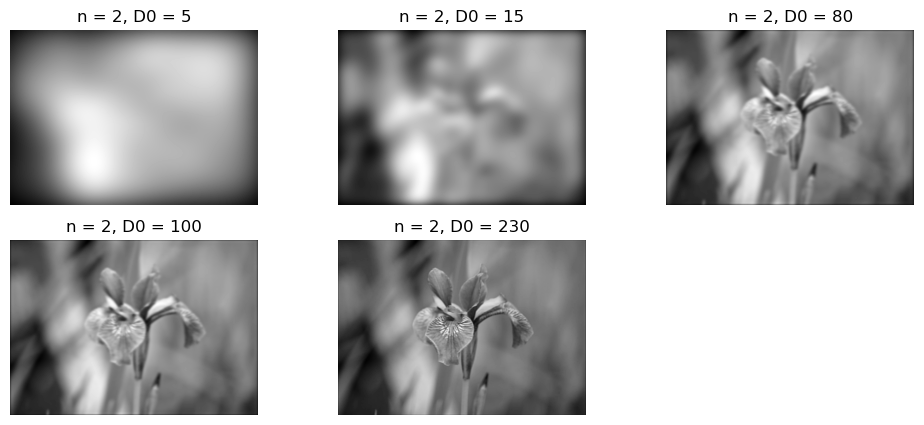
\includegraphics[width = \linewidth]{fo16.png}
        \caption{Kết quả của Butterworth Low-Pass Filter, padding size*2, keep the order, change the distance}
        \label{fig17}
        \end{figure}
        \phantom{a}\\
        Hình \ref{fig18} thì ngược lại.
        \begin{figure}[ht!]
        \centering
        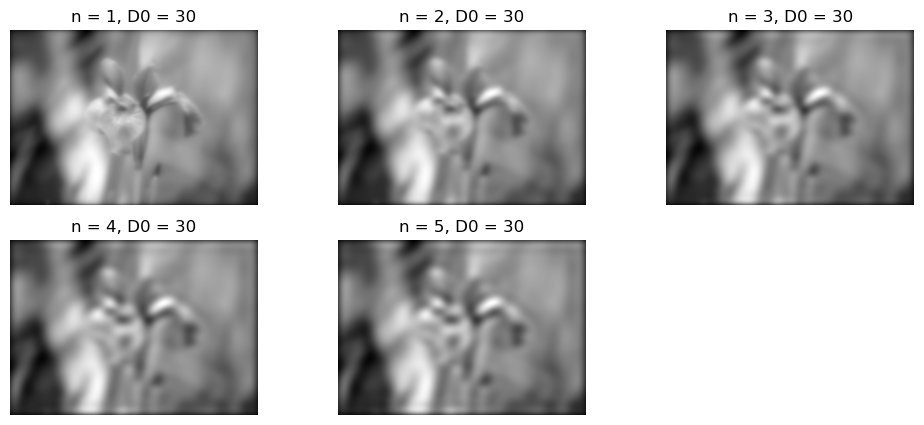
\includegraphics[width = \linewidth]{fo17.png}
        \caption{Kết quả của Butterworth Low-Pass Filter, padding size*2, keep the distance change the order}
        \label{fig18}
        \end{figure}
        
        \newpage
        \phantom{a}
        \newpage
        \subsection{High-Pass Filtering}
        Trực quan thì bộ lọc thông-cao là phần bù của lọc thông thấp, ý nghĩa cũng xuất phát từ cái tên, chỉ cho những thành phần có tần số cao qua, và loại bỏ những thành phần có tần số thấp. Đôi khi đơn giản, ta có thể suy ra bộ lọc thông-cao từ bộ lọc thông thấp qua công thức:
        $$ H_{HP} = 1 - H_{LP}$$
        và ngược lại.
        \subsubsection{Ideal High-Pass Filters}
        Hàm truyền của \textit{Ideal High-Pass Filters}:
        $$
        H(u,v) = \begin{cases}
            0, \phantom{a}if D(u,v) \leq D_0\\
            1,\phantom{a} if D(u,v) > D_0
        \end{cases}
        $$
        \begin{figure}[ht!]
        \centering
        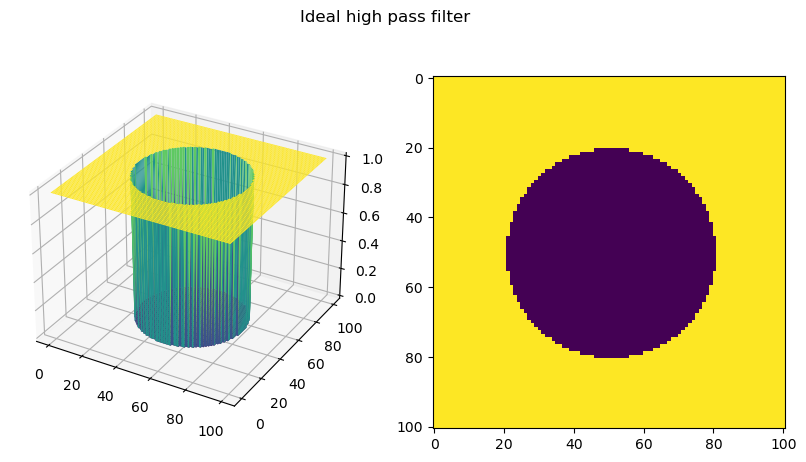
\includegraphics[width = \linewidth]{fo18.png}
        \caption{Ideal High-Pass Filter}
        \label{fig19}
        \end{figure}
        Hình \ref{fig20} cho ta kết quả của bộ lọc thông-cao lí tưởng.
         \begin{figure}[ht!]
        \centering
        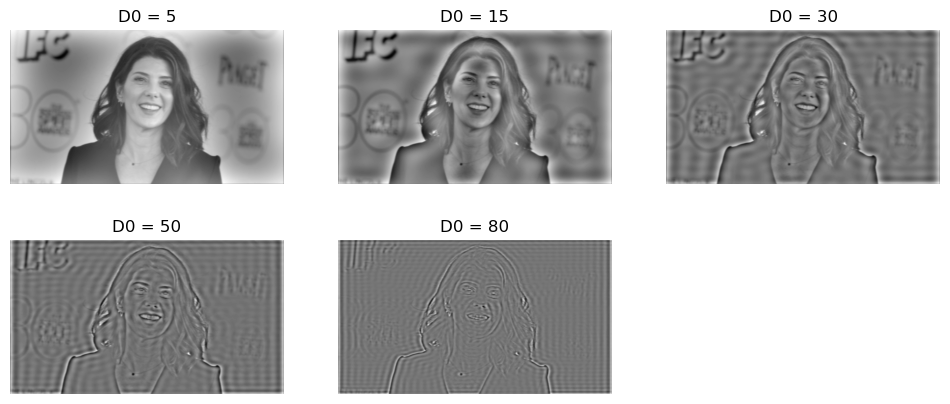
\includegraphics[width = \linewidth]{fo19.png}
        \caption{Kết quả của Ideal High-Pass Filter, padding size*2}
        \label{fig20}
        \end{figure}

        \newpage
        \subsubsection{Gaussian High-Pass Filters}
        Hàm truyền có thể được cho bởi:
        $$H(u,v) = 1-e^{-D^2(u,v)/2{D_0}^2}$$
        \begin{figure}[ht!]
        \centering
        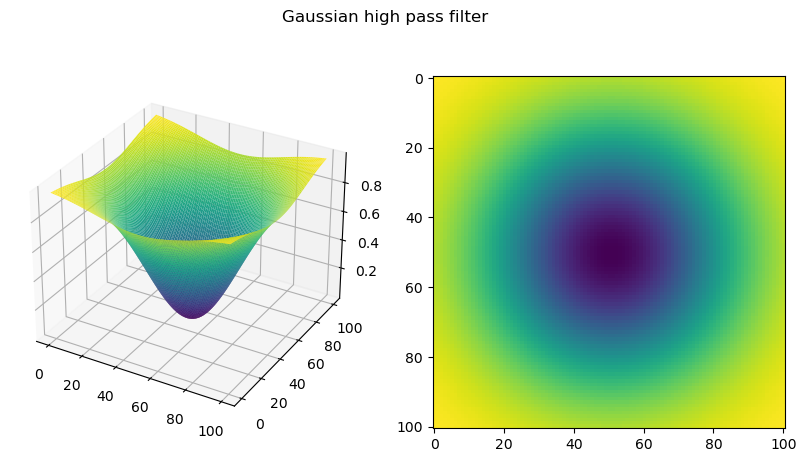
\includegraphics[width = \linewidth]{fo20.png}
        \caption{Gaussian High-Pass Filter}
        \label{fig21}
        \end{figure}
        Hình \ref{fig21} cho ta kết quả của bộ lọc thông-cao \textit{Gauss}.
         \begin{figure}[ht!]
        \centering
        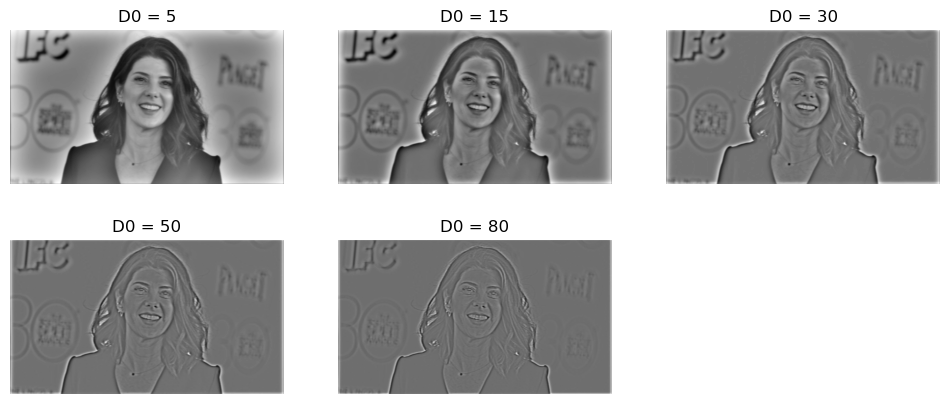
\includegraphics[width = \linewidth]{fo21.png}
        \caption{Kết quả của Gaussian High-Pass Filter, padding size*2}
        \label{fig22}
        \end{figure}
        
        
        \subsubsection{Butterworth High-Pass Filters}
        Hàm truyền được có thể được cho bởi công thức:
        $$H(u,v) = \frac{1}{1+\left[D_0/D(u,v)\right]^{2n}}$$
        \begin{figure}[ht!]
        \centering
        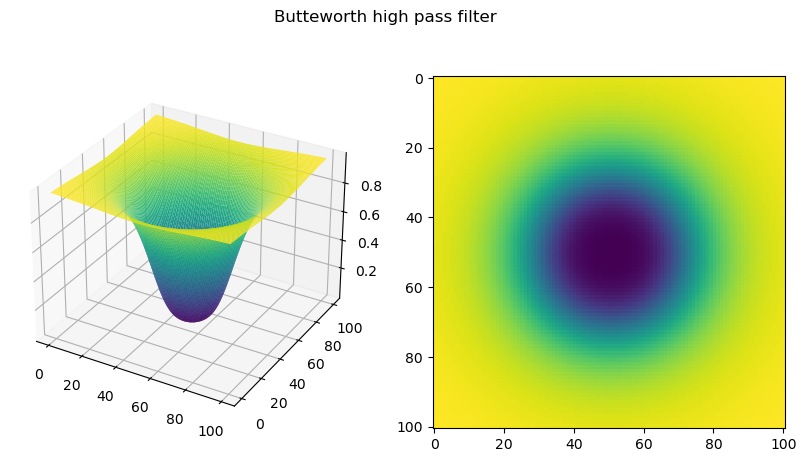
\includegraphics[width = \linewidth]{fo22.png}
        \caption{Butterworth High-Pass Filter}
        \label{fig23}
        \end{figure}
        Hình \ref{fig24} cho ta kết quả của \textit{Butterworth High-Pass Filtering} khi giữ cấp độ và thay đổi các khoảng cách.
        \begin{figure}[ht!]
        \centering
        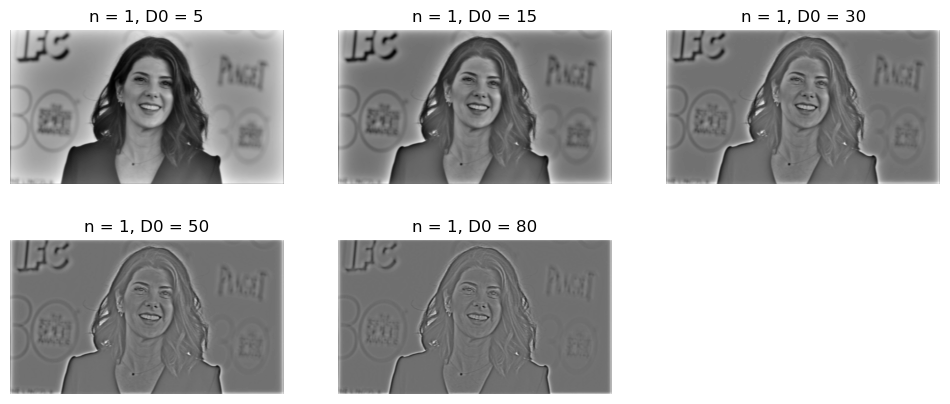
\includegraphics[width = \linewidth]{fo23a.png}
        \caption{Kết quả của Butterworth High-Pass Filter, padding size*2, keep the order, change the distance}
        \label{fig24}
        \end{figure}
        \phantom{a}\\
        Hình \ref{fig25} thì ngược lại.
        \begin{figure}[ht!]
        \centering
        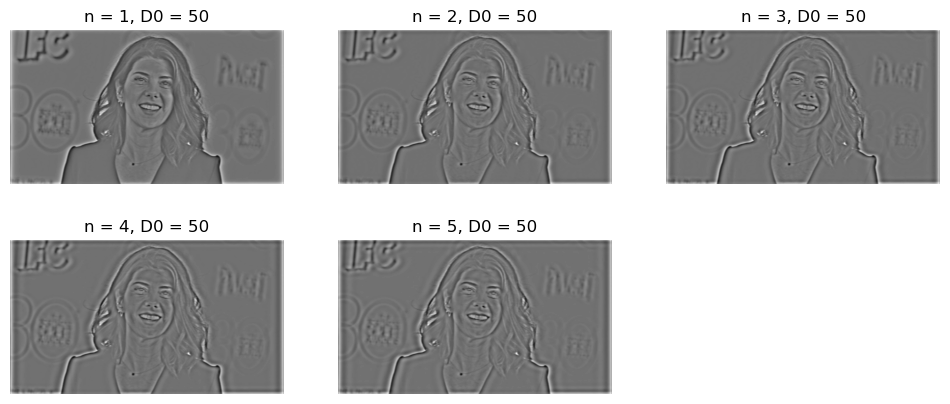
\includegraphics[width = \linewidth]{fo23b.png}
        \caption{Kết quả của Butterworth High-Pass Filter, padding size*2, keep the distance change the order}
        \label{fig25}
        \end{figure}

        \newpage
        \phantom{a}
        \newpage
        \subsubsection{Làm nét ảnh?}
        Bạn có thấy ảnh của bộ lọc thông-cao thường tối và chỉ hiện một lượng ít thông tin của bức ảnh? Tuy ít nhưng nó rất đáng giá đấy! Bởi, cạnh và các chi tiết nhỏ của ảnh là những thành phần tần số cao! Qua đây, câu hỏi đặt ra: Liệu ta có thể làm nét ảnh bằng cách cộng ảnh như đã làm với \textit{bộ lọc Laplace} trong bài trước? Tôi đoán là có! Đây là những hình ảnh minh chứng cho việc đó!
        \begin{figure}[ht!]
            \centering
            \begin{subfigure}[b]{0.7\linewidth}
                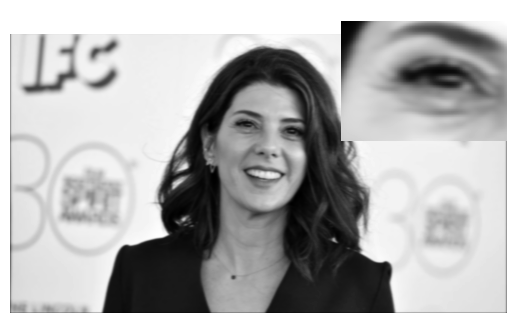
\includegraphics[width=\linewidth]{fo24a.png}
                \caption{Ảnh mờ gốc, lấy từ Gauss}
            \end{subfigure}
            \begin{subfigure}[b]{0.45\linewidth}
                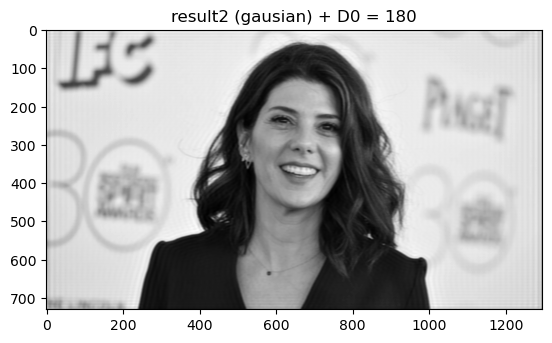
\includegraphics[width = \linewidth]{fo24b.png}
                \caption{Làm nét bằng Ideal High-Pass Filter}
            \end{subfigure}
            \begin{subfigure}[b]{0.45\linewidth}
                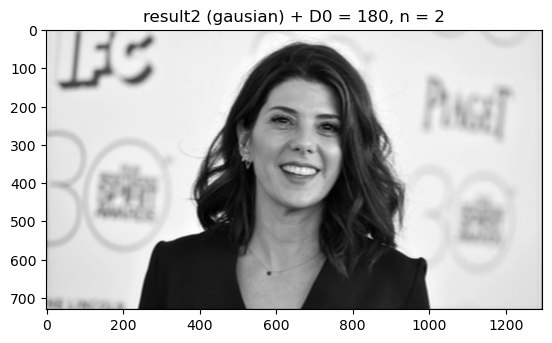
\includegraphics[width=\linewidth]{fo24c.png}
                \caption{Làm nét bằng Butterworth High-Pass Filter}
            \end{subfigure}
            \begin{subfigure}[b]{0.45\linewidth}
                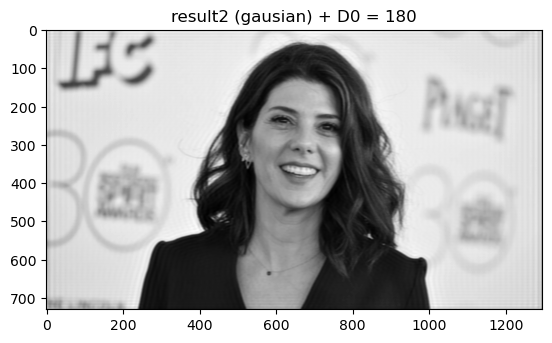
\includegraphics[width=\linewidth]{fo24b.png}
                \caption{Làm nét bằng Gaussian High-Pass Filter}
            \end{subfigure}
            \caption{Làm nét bằng High-Pass Filters}
            \label{fig26}
        \end{figure}
        \begin{figure}
            \centering
            \begin{subfigure}[b]{0.9\linewidth}
                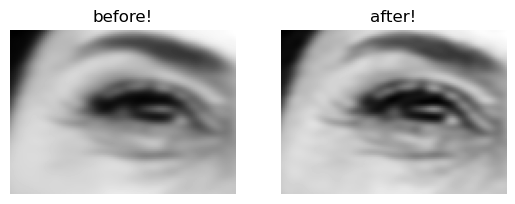
\includegraphics[width = \linewidth]{fo25a.png}
                \caption{Làm nét bằng Ideal High-Pass Filter}
            \end{subfigure}
            \begin{subfigure}[b]{0.9\linewidth}
                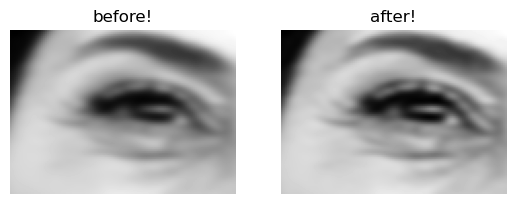
\includegraphics[width=\linewidth]{fo25b.png}
                \caption{Làm nét bằng Butterworth High-Pass Filter}
            \end{subfigure}
            \begin{subfigure}[b]{0.9\linewidth}
                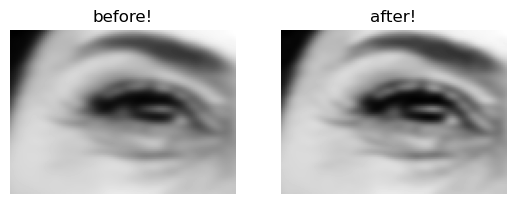
\includegraphics[width=\linewidth]{fo25c.png}
                \caption{Làm nét bằng Gaussian High-Pass Filter}
            \end{subfigure}
            \caption{Rõ ràng hơn!}
            \label{fig27}
        \end{figure}
        \\Hình \ref{fig26} và Hình \ref{fig27}.
        \subsubsection{Thảo luận}
        Tại sao khi cộng ảnh lại ra ảnh nét hơn? Tôi đoán, sau khi ta cộng ảnh, cường độ ảnh tại những thành phần có tần số cao sẽ lớn hơn, điều này khiến những đường viền (\textit{cạnh - edges}) trở nên rõ ràng hơn! Ta có thể can thiệp vào việc này dựa cấp độ (\textit{$n$ hoặc $D_0$}) của bộ lọc!
        
        \newpage
        \phantom{a}
        \newpage
        \section{Mã nguồn}
        Mã nguồn cho bài này có thể tìm thấy ở đây:
        \href{https://github.com/thuantn210823/Computer-Vision-IPSAL-LAB-}{My github}\\ Mọi thắc mắc, ý kiến đóng góp liên hệ: \emph{email: thuan.tn210823@sis.hust.edu.vn}
        \section{Tài liệu tham khảo}
        \begin{thebibliography}{9}
        \bibitem{slide}
    Truong. PV, Thao. TT \emph{Silde bài giảng tuần 4}, Đại học Bách Khoa Hà Nội.
        \bibitem{book}
        Liem. NX \emph{Giải tích - Tập hai}, Nhà xuất bản giáo dục - 1998.
        \bibitem{book}
        Phuoc. ND \emph{Lý thuyết Điều khiển tuyến tính, tái bản lần hai}, Nhà xuất bản khoa học và kĩ thuật - 2005.
        \bibitem{book}
    R.C. Gonzalez and R.E. Woods \emph{Digital image processing ($3^{rd}$ editon)}, Prentice Hall, 2008.

    \bibitem{website}
    \href{https://math.libretexts.org/Bookshelves/Differential_Equations/Introduction_to_Partial_Differential_Equations_(Herman)/09%3A_Transform_Techniques_in_Physics/9.02%3A_Complex_Exponential_Fourier_Series}{Complex Exponential Fourier Series - Math.libretexts.org.}
    \bibitem{website}
    \href{https://www.tutorialspoint.com/derivation-of-fourier-transform-from-fourier-series}{Derivation of Fourier Transform from Fourier Series - Tutorialspoint.com.}
    \bibitem{website}
    Wikipedia \href{https://vi.wikipedia.org/wiki/Joseph_Fourier}{Josehp Fourier.}
    \end{thebibliography}
\end{document}
